%! Author = lazza
%! Date = 28/05/2022

\section{MIMD}\label{sec:mimd}
The execution can be synchronous or asynchronous, deterministic or non-deterministic.

\paragraph{Advantages:} \textbf{Multipurpose} processor that can be built starting from \textbf{standard CPUs} (often
off-the-shelf
microprocessors) that act independently one from the other: each processor fetches its own instructions and operates
on its own data.
\textbf{Scalable} to a variable number of processor nodes.\\
\textbf{Flexible:}
\begin{itemize}
    \item single-user machines focusing on high-performance for one
    specific application
    \item multi-programmed machines running many tasks
    simultaneously
    \item some combination of these functions.
\end{itemize}
\textbf{Cost/performance} advantages due to the use of off-
the-shelf microprocessors these can be combined in the same system.

\paragraph{Disadvantage:} Fault tolerance issues.

\paragraph{Exploting MIMD} To exploit a MIMD with $n$ processors, we need:
\begin{itemize}
    \item at least $n$ threads or processes to execute
    \item independent threads typically identified by the programmer or
    created by the compiler
    \item parallelism is contained in the threads \textrightarrow thread-level parallelism
\end{itemize}

\textbf{Note:} parallelism is identified by the software.\\

\subsection{MIMD machines classes}\label{subsec:mimd-machines}
Existing MIMD machines fall into 2 classes, depending on the number
of processors involved, which in turn dictates a memory organization
and interconnection strategy.

\paragraph{Key design issues}
\begin{itemize}
    \item how many processors?
    \item how powerful are processors?
    \item how do parallel processors share data?
    \item where to place the physical memory?
    \item how do parallel processors cooperate and coordinate?
    \item what type of interconnection topology?
    \item how to program processors?
    \item how to maintain cache coherency?
    \item how to maintain memory consistency?
    \item how to evaluate system performance?
\end{itemize}

\subsubsection{Centralized shared-memory architectures}\label{subsubsec:centralized-shared-memory-architectures}
\begin{itemize}
    \item at most few dozen processor chips (< 100 cores)
    \item large caches, single memory multiple banks
    \item often called symmetric multiprocessors (SMP) and the
    style of architecture called Uniform Memory Access (UMA)
\end{itemize}

\begin{figure}[h]
    \centering
    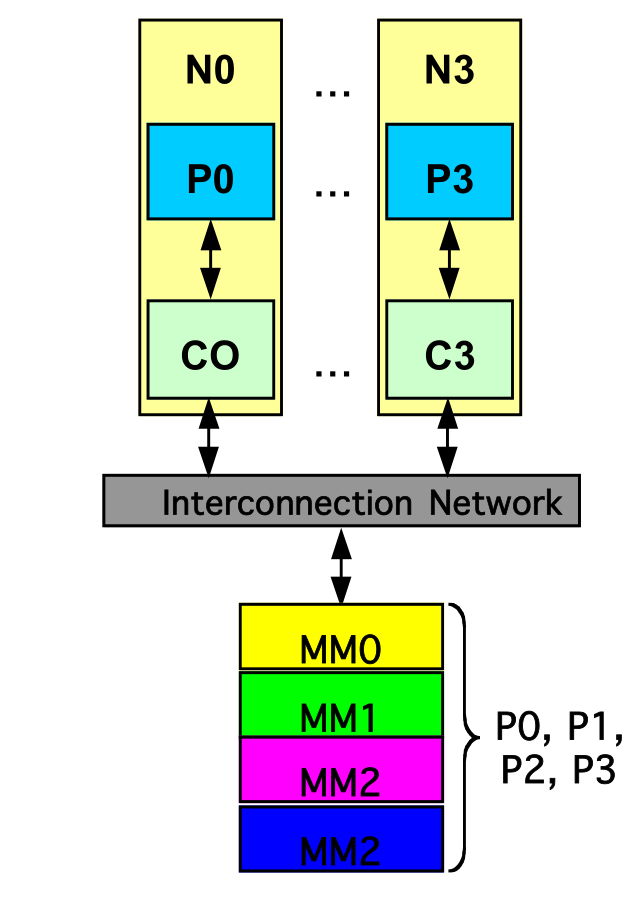
\includegraphics[scale = 0.2]{images/centralized-shared-memory-architectures}
    \caption{Shared memory architecture}
    \label{fig:centralized-shared-memory-architectures}
\end{figure}

\subsubsection{Distributed memory architectures}\label{subsubsec:distributed-memory-architectures}
\begin{itemize}
    \item to support large processor counts
    \item requires high-bandwidth interconnect
    \item disadvantage: need of data communication among processors
    \item Non Uniform Memory Access (NUMA)
\end{itemize}

\begin{figure}[h]
    \centering
    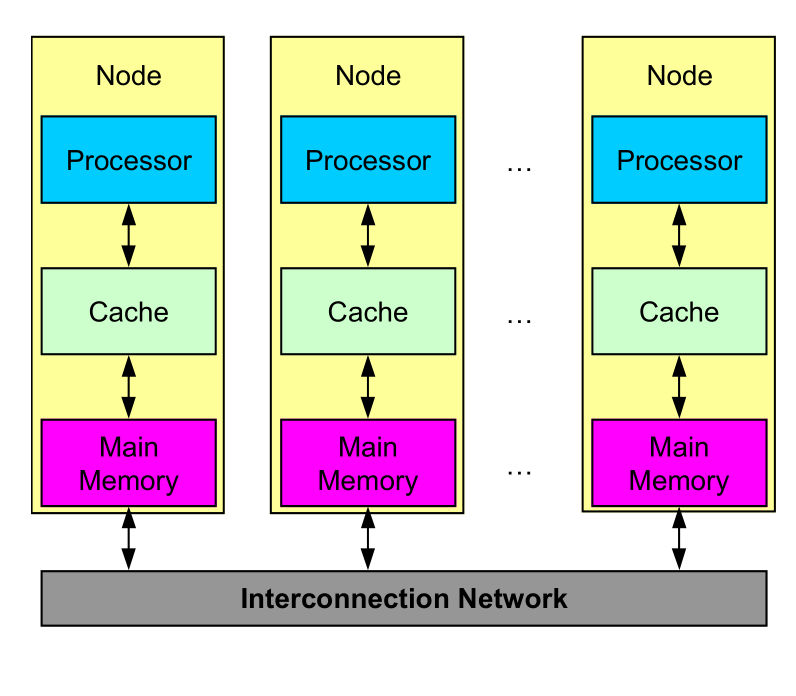
\includegraphics[scale = 0.2]{images/distributed-memory-architectures}
    \caption{Distributed memory architectures}
    \label{fig:distributed-memory-architectures}
\end{figure}

\paragraph{Tile64} is a VLIW ISA multicore processor manufactured by Tilera.
It consists of a mesh network of 64 "tiles", where each tile houses a general purpose processor, cache,
and a non-blocking router, which the tile uses to communicate with the other tiles on the processor.
The short-pipeline, in-order, three-issue cores implement a MIPS-inspired VLIW instruction set.
Each core has a register file and three functional units: two integer arithmetic logic units and a load-store unit.
Each of the cores ("tile") has its own L1 and L2 caches plus an overall virtual L3 cache which is an aggregate of all
the L2 caches.
A core is able to run a full operating system on its own or multiple cores can be used to run a symmetrical
multi-processing operating system.

\begin{figure}[h]
    \centering
    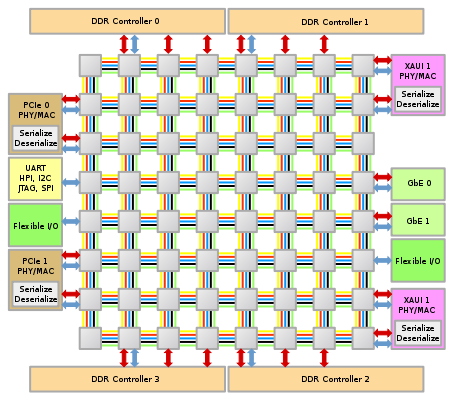
\includegraphics[scale = 0.4]{images/Tile64}
    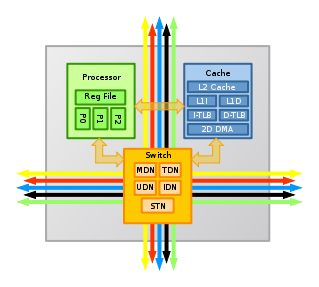
\includegraphics[scale = 0.5]{images/Tile64-Tile}
    \caption{Tile64}
    \label{fig:tile64}
\end{figure}


\subsubsection{Examples}\label{subsubsec:examples}

\paragraph{Cell: PS3}
Cell is a heterogeneous chip multiprocessor:
\begin{itemize}
    \item One 64-bit Power core
    \item 8 specialized co-processors\\
    \textrightarrow based on a novel single-instruction multiple-data (SIMD)
    architecture called SPU (Synergistic Processor Unit)
\end{itemize}

\paragraph{Xenon: XBOX360}
Xenon is a homogeneous chip multiprocessor:
\begin{itemize}
    \item three symmetrical cores, each two way SMT-capable and clocked at 3.2 GHz
    \item SIMD: VMX128 extension for each core
    \item 1 MMB L2 cache (lockable by the GPU) running at half-speed (1.6 GHz) with a 256-bit bus
\end{itemize}

Microsoft envisions a procedurally rendered game
as having at least two primary components:
\begin{itemize}
    \item Host thread: a game's host thread will contain the main
thread of execution for the game
    \item Data generation thread: where the actual procedural
synthesis of object geometry takes place
\end{itemize}
These two threads could run on the same PPE, or
they could run on two separate PPEs.
In addition to the these two threads, the game
could make use of separate threads for handling
physics, artificial intelligence, player input, etc.


\subsection{Procedural synthesis}\label{subsec:procedural-synthesis}
Procedural synthesis about making optimal use of system bandwidth
and main memory by dynamically generating lower-level geometry
data from statically stored higher-level scene data.

\begin{figure}[h]
    \centering
    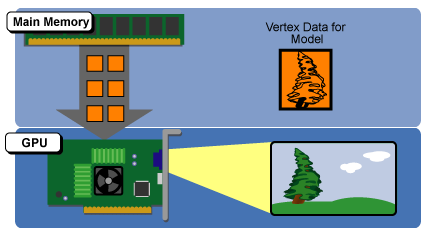
\includegraphics[scale = 0.]{images/procedural-synthesis}
    \caption{Procedural synthesis}
    \label{fig:procedural-synthesis}
\end{figure}

For 3D games:
\begin{itemize}
    \item Artists use a 3D rendering program to produce content for the game
    \item Each model is translated into a collection of polygons
    \item Each polygons is represented in the computer's memory as collections of vertices
\end{itemize}
When the computer is rendering a scene in a game in real-time:
\begin{itemize}
    \item Models that are being displayed on the screen start out in main
memory as stored vertex data
    \item That vertex data is fed from main memory into the GPU where it is then rendered into a 3D image and output
    to the monitor as a sequence of frames.
\end{itemize}

\paragraph{Limitations} there are two problems:
\begin{itemize}
    \item The costs of creating art assets for a 3D game are
going through the roof along with the size and
complexity of the games themselves
    \item Console hardware's limited main memory sizes and
limited bus bandwidth
\end{itemize}


\subsection{Memory Address Space Model}\label{subsec:memory-address-space-model}
How do parallel processors share data?
We already talked about how the physical memory implementation divides the \textit{machines} in two classes, now we 
look how the virtual memory is from the perspective of a process.

\subsubsection{Single logically shared address space}
A memory reference can be made by any processor to any memory location, this model adapts well to the
\textit{shared memory architectures}: the address space is shared among processors, the same physical address on 2
processors refers to the same location in memory.

\begin{figure}[h]
    \centering
    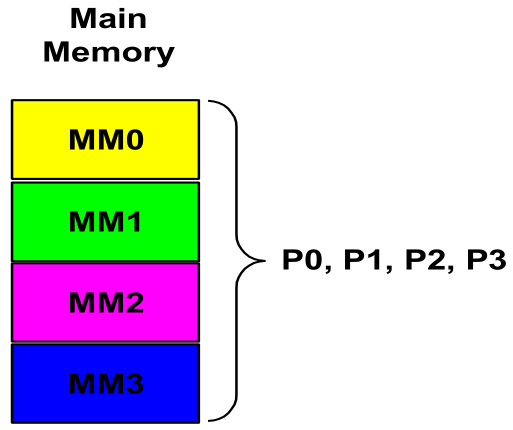
\includegraphics[scale = 0.3]{images/single-logically-shared-address-space}
    \caption{Single logically shared address space}
    \label{fig:single-logically-shared-address-space}
\end{figure}

\paragraph{Shared Address}
\begin{itemize}
    \item the processors communicate among them through shared variables in memory
    \item implicit management of the communication through load/store operations to access any memory locations
    \item shared memory does not mean that there is a single centralized memory
\end{itemize}

\subsubsection{Multiple and private address spaces}
The processors communicate among them through send/receive primitives, this model adapts well to \textit{message
passing architectures}: the address space is logically disjoint and cannot be addressed by different processors, the
same physical address on 2 processors refers to 2 different locations in two different memories.

\begin{figure}[h]
    \centering
    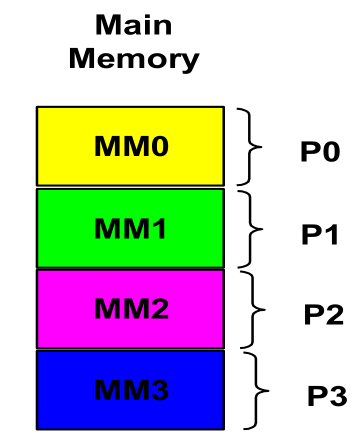
\includegraphics[scale = 0.3]{images/multiple-and-private-address-spaces}
    \caption{Multiple and private address spaces}
    \label{fig:multiple-and-private-address-spaces}
\end{figure}

\paragraph{Private address}
\begin{itemize}
    \item the processors communicate among them through sending/receiving messages
    \item explicit management of the communication through send/receive primitives to access private memory locations
    \item no cache coherency problem among processors
\end{itemize}

\textbf{Note:} The concepts of addressing space
(single/multiple) and the physical memory
organization (centralized/distributed) are
orthogonal to each other: they could be combined freely.
Multiprocessor systems can have single
addressing space and distributed physical
memory.

\begin{figure}[h]
    \centering
    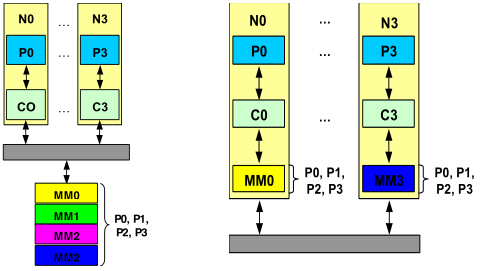
\includegraphics[scale = 0.43]{images/address-space-vs-physical-memory-org}
    \caption{Single shared space vs physical memory}
    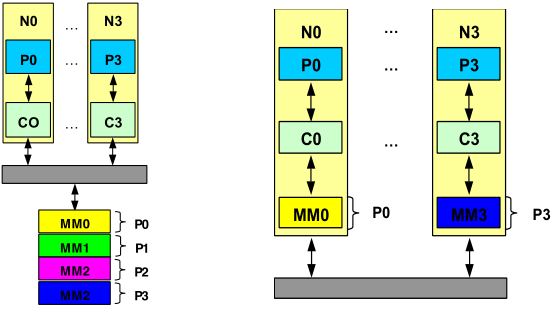
\includegraphics[scale = 0.40]{images/address-space-vs-physical-memory-org-1}
    \caption{Multiple private addresses vs physical memory }
    \label{fig:address-space-vs-physical-memory-org}
\end{figure}


\subsection{Programming Model}\label{subsec:programming-model}

\subsubsection{Shared Memory}
The program is a collection of threads of control, each thread:
\begin{itemize}
    \item can be created dynamically, mid execution, in some languages.
    \item has a set of \textit{private} variables, e.g., local stack variables
    \item also a set of \textit{shared} variables, e.g., static variables, shared common blocks, or global heap
\end{itemize}

Processes communication:
\begin{itemize}
    \item implicitly by writing and reading shared variables
    \item coordination by synchronizing on shared variables
\end{itemize}

\begin{figure}[h]
    \centering
    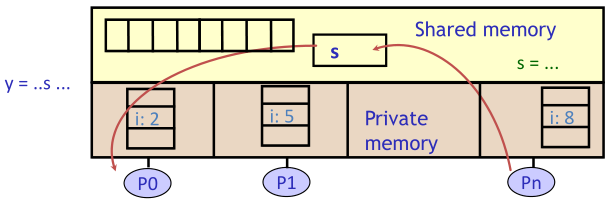
\includegraphics[width = \linewidth]{images/shared-memory-model}
    \caption{Shared memory}
    \label{fig:shared-memory-model}
\end{figure}

\paragraph{Advantages}
\begin{itemize}
    \item implicit communication (loads/stores)
    \item low overhead when cached
\end{itemize}

\paragraph{Disadvantages}
\begin{itemize}
    \item complex to build in way that scales well -- e.g., distance between core and memory may become too much
    cutting down performance
    \item requires synchronization operations
    \item hard to control data placement within caching system
\end{itemize}

\subsubsection{Message Passing}
The program consist of a collection of \textbf{named} processes:
\begin{itemize}
    \item usually fixed at program startup time
    \item thread of control plus local address space, no shared data
    \item logically shared data is partitioned over local processes
\end{itemize}

Processes communication:
\begin{itemize}
    \item explicitly by send/receive pairs
    \item coordination is implicit in every communication event
    \item MPI (Message Passing Interface) is the most commonly used SW
\end{itemize}

\begin{figure}[h]
    \centering
    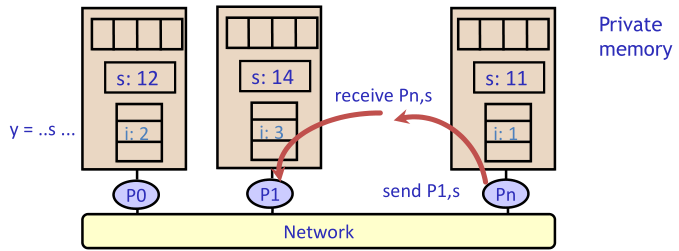
\includegraphics[width = \linewidth]{images/message-passing-model}
    \caption{Message passing}
    \label{fig:message-passing-model}
\end{figure}

\paragraph{Advantages}
\begin{itemize}
    \item explicit communication (sending/receiving of messages)
    \item easier to control data placement (no automatic caching)
\end{itemize}

\paragraph{Disadvantages}
\begin{itemize}
    \item message passing overhead can be quite high
    \item more complex to program
    \item introduces question of reception technique (interrupts/polling)
\end{itemize}

\paragraph{Massively Parallel Processors Problems}
\begin{itemize}
    \item all data must be handled by software: cannot retrieve remote data except with message request/reply
    \item message passing has high software overhead:
    \begin{itemize}
        \item early machine had to invoke OS on each message
        \item even user level access to network interface has dozens of cycle overhead
        \item sending messages can be cheap (just like stores)
        \item receiving messages is expensive, need to poll or interrupt
    \end{itemize}
\end{itemize}